%%%%%%%%%%%%%%%%%%%%%%%%%%%%%%%%%%%%%%%%%%%%%%%%%%%%%%%%%%%%%%%%%%%%%%%%%%%%%%%%
%2345678901234567890123456789012345678901234567890123456789012345678901234567890
%        1         2         3         4         5         6         7         8

\documentclass[letterpaper, 10 pt, conference]{ieeeconf}  % Comment this line out if you need a4paper

%\documentclass[a4paper, 10pt, conference]{ieeeconf}      % Use this line for a4 paper

\IEEEoverridecommandlockouts                              % This command is only needed if 
                                                          % you want to use the \thanks command

\overrideIEEEmargins                                      % Needed to meet printer requirements.

% See the \addtolength command later in the file to balance the column lengths
% on the last page of the document

% The following packages can be found on http:\\www.ctan.org
\usepackage{graphicx} % for pdf, bitmapped graphics files
%\usepackage{epsfig} % for postscript graphics files
%\usepackage{mathptmx} % assumes new font selection scheme installed
%\usepackage{times} % assumes new font selection scheme installed
\usepackage{amsmath} % assumes amsmath package installed
\usepackage{amssymb}  % assumes amsmath package installed

\usepackage{subfigure}


\title{Encounter Based Multi Robot Simultaneous Localization and Occupancy Grid Mapping}


% author names and affiliations
% use a multiple column layout for up to three different
% affiliations
\author{RB Choroszucha$^{1}$, C Hyman$^{2}$, and A Collier$^{3}$ % <-this % stops a space
\thanks{$^{1}$ RB Choroszucha is with the School of Naval Architecture and Marine Engineering, University of Michigan.  E-mail: riboch{@}umich.edu}%
\thanks{$^{2}$ C Hyman is with the School of Electrical Engineering and Computer Science, University of Michigan. E-mail: {hymanc}{@}umich.edu}
\thanks{$^{3}$ A Collier is with the School of Electrical Engineering and Computer Science, University of Michigan. E-mail: {amcollie}{@}umich.edu}
}



\begin{document}



\maketitle
\thispagestyle{empty}
\pagestyle{empty}


%%%%%%%%%%%%%%%%%%%%%%%%%%%%%%%%%%%%%%%%%%%%%%%%%%%%%%%%%%%%%%%%%%%%%%%%%%%%%%%%
\begin{abstract}

In this paper we present and implement the algorithm in Howard's 2006 paper: ``Multi-robot simultaneous localization and mapping using particle filters.''  While Howard's method is attractive for its speed, it only uses a single particle filter for all the robots which can result in undesired particle error and depletion.  In this paper we propose a modification of the algorithm to using independent particle filters for each robot, and demonstrate the efficacy of the technique on a simulated data set.  

\end{abstract}

\section{Introduction}
\label{S:Intro}


The automated exploration of unknown environments has become one of the foremost challenges in mobile robotics. For a robot to explore an environment, it must map the environment and concurrently localize itself within the environment.  The framework used to perform this task is known as simultaneous localization and mapping (SLAM) and has been well covered in the literature using a variety of techniques \cite{durrant2006simultaneous,bailey2006simultaneous}.

While SLAM is well known and has a rich history of successes using a single robot, it can often be a slow process due to both constraints on the robot, such as speed and data processing, and lack of redundancy, i.e. robot failure \cite{thrun2001probabilistic,burgard2005coordinated}.  To address the speed of mapping and to add redundancy, coordinated or multi-robot SLAM (MRSLAM) was created.

MRSLAM is as it sounds, SLAM using multiple exploring robots. This approach allows for the partition of the physical search space using different robots, typically decreasing the time it takes to map an area, and increasing the likelihood of full map coverage in the event of robot failure. This temporal exploration parallelism does, however, come at the cost of added complexity. The added complexity of MRSLAM comes in two major components: coordination of exploration using multiple search agents and merging the maps of these agents \cite{fox2006distributed}.  Coordinated exploration consists of planning the groups' search path, most often formulated to cover the most search space in minimum time or to optimize some other mapping cost criteria. The other major component, map merging, is the combination of individual robot's observations and maps into one cohesive global map estimate.

In this paper we use the map merging algorithm presented in Howard's 2006 paper: ``Multi-Robot Simultaneous Localization and Mapping using Particle Filters'' \cite{howard2006multi} to build an occupancy grid of a defined space. This paper is of particular interest as it presents a resource efficient online solution to the MRSLAM map merging problem given unknown initial robot poses.  

The algorithm presented is an encounter-based algorithm.  Given that we start with one mapping robot (call this Robot 1), when it encounters another robot (Robot 2), the relative pose between the two robots is computed and Robot 2's odometry and scan data is transmitted in reverse order to Robot 1, where the data is integrated to create a single map posterior.

Fig. \ref{fig:HowardFig3} depicts the process with robot 1's Pose-Actuator-Sensor triple $(x^1_t,u^1_{t-1},z^1_t)$ (PAS triple), and robot 2's PAS triple $(x^2_t,u^2_{t-1},z^2_t)$.
When $t=2$, robot 1 observes robot 2 and determines the relative pose $\Delta$, then the past odometry and scan data is integrated in reverse order.

\begin{figure}[h]
\centering
\includegraphics[width=\columnwidth]{{{../FinalFigures/HowardFig3}}}
\caption{Depiction of data integration. Taken from \cite{howard2006multi}.}
\label{fig:HowardFig3}
\end{figure}

The paper is structured as follows: In \S\ref{S:Back} some background about MRSLAM is provided, the contribution of \cite{howard2006multi} and the modified algorithm is discussed .  In \S\ref{S:Alg} the algorithm of \cite{howard2006multi}, and its modification, is presented.  In \S\ref{S:Exp}, the two algorithms are compared qualitatively using a simulated data set. 



\section{Background}
\label{S:Back}

\subsection{State of the Art}
\label{SS:Back:SOA}
    
In the literature there are two problems that are often addressed when dealing with MRSLAM:
\begin{enumerate}
\item robot coordination, i.e., how to cover the most area given an unknown environment \cite{julia2012comparison}, and
\item merging the data to create one global map posterior, which is what we will focus on.
\end{enumerate}

In the case where all relative robot poses are known, merging maps is a trivial problem using small modifications to existing SLAM techniques \cite{thrun2001probabilistic}. In the general MRSLAM problem, however, robots may start with unknown absolute and relative poses, and therefore merging of maps requires the discovery of relative relationships between different robot trajectories to build a single map. This is often a costly process, which in general can be solved for robots sharing a search space by estimating each robot's relative pose given a partial map, but this leads to exponential complexity with respect to the number of exploring robots \cite{fox2006distributed}. Nevertheless, several practical algorithms exist to circumvent this naive and inefficient approach,  including coarse topological matching and stitching techniques borrowed from computer vision \cite{birk2006merging}.


A majority of the papers employ a Rao-Blackwellized particle filter (RBPF) for building occupancy grids.  


\cite{howard2006multi,birk2006merging,lazaro2013multi,lee2012probabilistic}


-What does the literature cover?

-Where did it begin, what did it progress to?




\subsection{\cite{howard2006multi} Extension to Original Work}
\label{SS:Back:Contributions}

\[
w_3^i=w_2^i w_1^i
\]


\begin{figure}[h]
\centering
\subfigure[Case where the peak weights are chosen, instead only mediocre points get the highest weighting.]{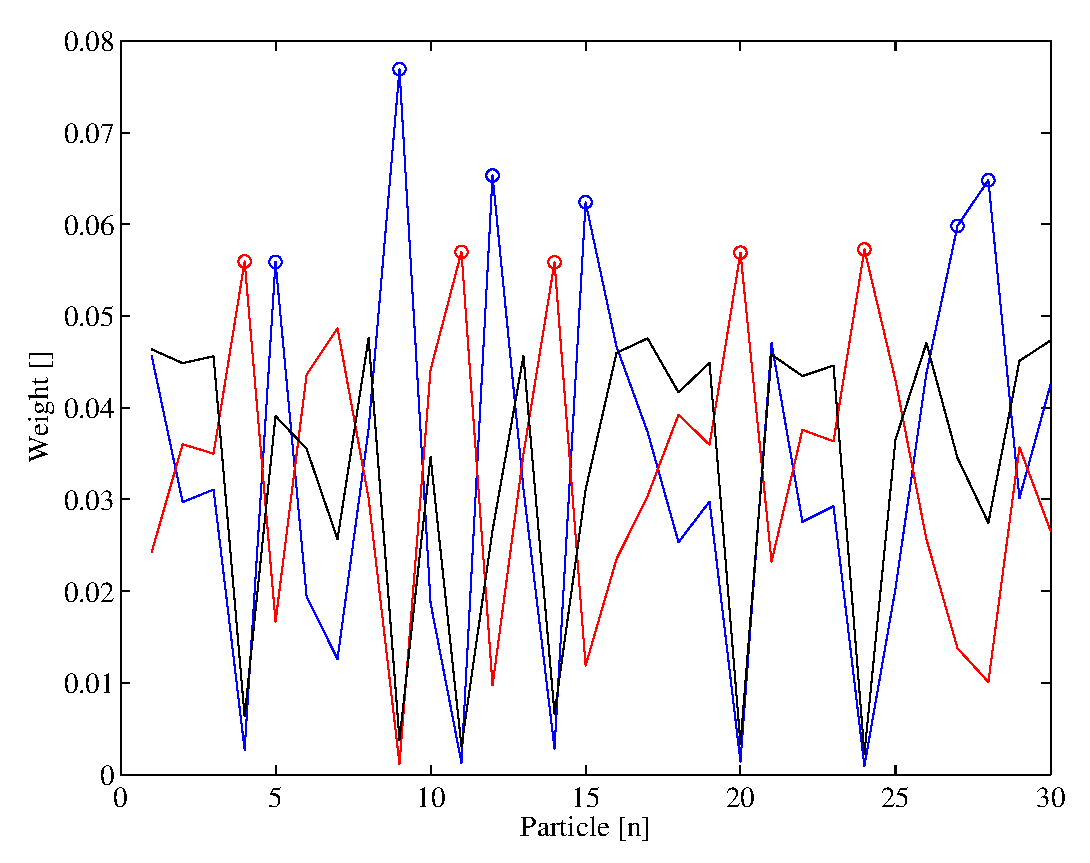
\includegraphics[width=\columnwidth]{../FinalFigures/Depletion}}
\subfigure[Forward (black) and reverse (red) model.  Simple pendulum with two different particle filters: the single particle filter that draws from  (circles), and the independent particle filters (squares).]{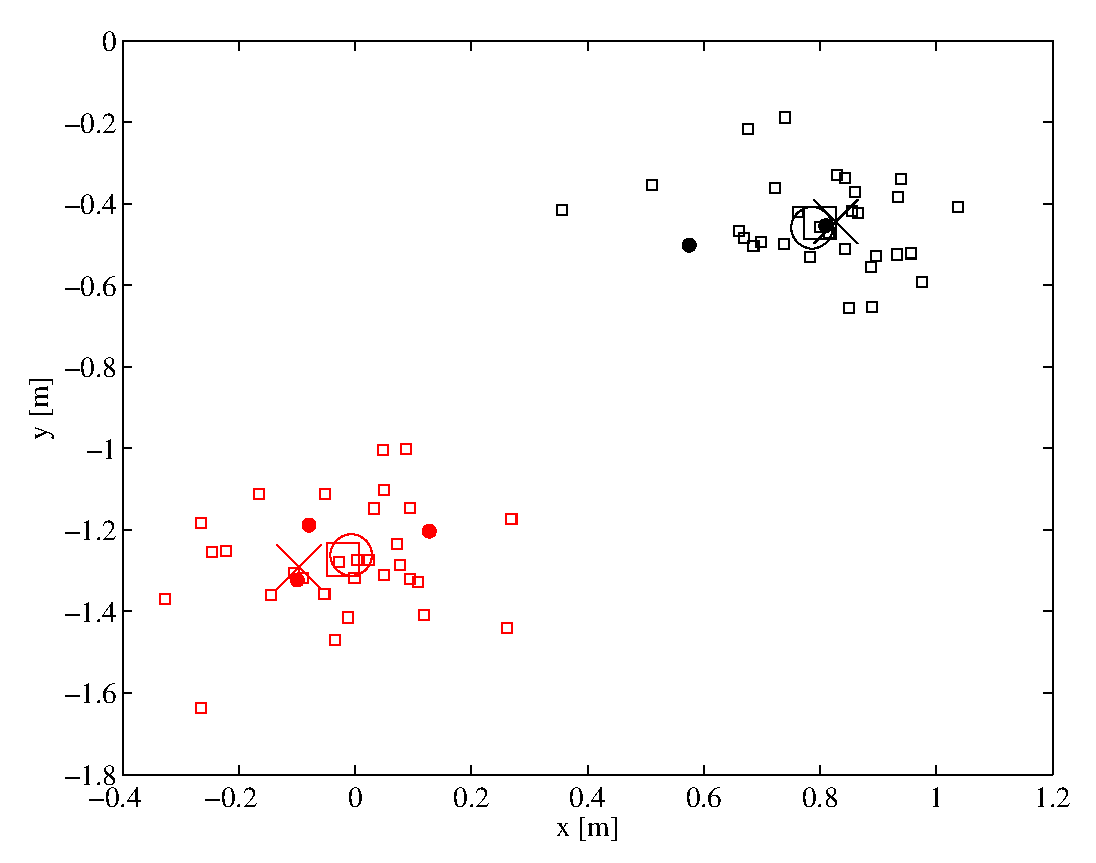
\includegraphics[width=\columnwidth]{../FinalFigures/IndependentlySampled}}
\caption{Example where the mediocre points of each set get chosen causing .}
\label{fig:deplete}
\end{figure}

While \cite{howard2006multi}

\section{The Algorithm}
\label{S:Alg}

\subsection{Overview}
\label{SS:Alg:Overview} 


Howard’s multi-robot SLAM algorithm generates a single map and pose posterior much in the same way an occupancy grid map SLAM algorithm based on a Rao-Blackwellized particle filter (RBPF) would, but with additions to accommodate multiple robots. Mapping begins with a set consisting of a single robot with known pose and an occupancy grid map of the environment is built as this robot traverses and measures it. The ultimate goal of the algorithm is to simultaneously compute for time $t$, the full SLAM posterior containing all robot pose trajectories $x_{1:t}^i$ and the global map $m_{1:t}$, given only a single known initial pose and sets of measurements
\begin{align*}
p(x_{1:t}^1,x_{1:t}^2&,...,x_{1:t}^M,m_{1:t}|\\&x_0^1,z_{1:t}^1,u_{0:t}^1,\Delta_s^2,z_{1:t}^2,u_{0:t}^2,\Delta_s^3,...,\Delta_s^M,z_{1:t}^M,u_{0:t}^M)
\end{align*}

The odometry and measurement data of all other robots is stored as it is collected, as it cannot contribute to the global map without a known relative pose linking it to the frame of the first robot. As the first robot encounters additional robots via a mutual pose observation, the newly observed robot is added to the set of mapping robots and its actions and the map is sequentially conditioned by its actions and measurements. From the point of observation, all future actions and measurements of the new robot are used to condition the map posterior, and likewise all of its previously stored actions and measurements are played back in reverse order from that point as a virtual robot. This information is then passed to a pair of new particle filters for the pose of these robots that contribute to the same global map. 

As further encounters occur between any robot, real or virtual, in the mapping set and a previously unseen robot, the previously unseen robot is added to the set of mapping robots and its measured relative pose is again used to establish a reference point with which its actions and measurements can condition the map posterior. Further mutual observations of two robots already in the mapping set are ignored for the sake of simplicity. This encounter-add process is continued recursively for all robots until all stored and future odometry and measurements are exhausted or all possible mapping robots have made an encounter with the mapping set. Beyond this point, the algorithm behaves as a normal RBPF with a stacked state containing pose posteriors of all robots in addition to the map.


This algorithm relies on a number of assumptions that are requisite for it to effectively solve the MRSLAM problem. Firstly, for all explored regions to count towards the map, each mapping robot must have encountered a robot that is an element of the mapping set in order to make a fully connected graph of robot poses, and therefore maximally complete map. Additionally, each robot pose trajectory is independent of all other trajectories such that motion or observation from one robot does not affect another outside of encounter events \cite{howard2006multi}.

\subsection{Algorithm Details}
\label{SS:Alg:Details}
Howard’s MRSLAM algorithm follows the basic structure of the below steps that perform data queueing, robot encounter management, and SLAM filter updates.
\begin{enumerate}
\item Queue measurement, odometry, and mutual observation (encounter) data
\item For all robots in the mapping set, take first element from queue and update SLAM filter
\item For all new encounters, split encountered queue at present time into causal and acausal queues and instantiate a new set of particles for the causal and acausal trajectory of the observed robot.
\item For all available acausal queues, remove last element and use it to update the SLAM filter for the corresponding acausal robot
\item If data includes a prior encounter with a robot not in the mapping set, instantiate a new set of particle for this robot and its acausal virtual self at its location and split the queue for that robot into a causal and acausal queues
\item Repeat until all data is consumed
\end{enumerate}
\vspace{0.1in}
\subsubsection{Data Queueing}
As each robot $R$ collects data, its current odometry $u_t^R$ and measurements $z_t^R$ are added to a running queue data structure before processing. An encounter flag $E_t^R$ and relative pose $\Delta_t^R$, if available, are also added to this queue. 
$$queue_{0:t}^R = append(queue_{0:t-1}^R, \{ u_t^R, z_t^R, E_t^R, \Delta_t^R \})$$
The storing of this data allows for either immediate use by particle filters for robots in the mapping set, or later joining or SLAM filtering after a future encounter with a mapping robot.
\vspace{0.1in}
\subsubsection{Encounters}
An encounter in this sense is defined as the observation of one robot by another mapping robot that produces a relative pose estimate between the robots of $\Delta$. For this implementation, it was assumed that the estimation of $\Delta$ was deterministic for the sake of demonstration and simplicity.

Upon an encounter at time $s$ between robot $A$ in the mapping set with a pose $x_s^A$ and a robot $B$ not in the set with a measured relative pose $\Delta_s^{AB}$, a reference frame pose for each particle $i$ of the newly observed robot is instantiated as causal particle posterior $x_s^{B(i)}$ and acausal particle pose posterior $\bar{x}_s^{B(i)}$ as:
\begin{align*}
x_s^{B(i)} &= x_s^{A(i)} \oplus \Delta_s^{AB} \\
\bar{x}_s^{B(i)} &= x_s^{A(i)} \oplus \Delta_s^{AB}
\end{align*}
Where $\oplus$ is the pose composition operator. <SSC reference?>
At this time, the stored data queue for robot B is also split into a causal queue $queue^B$ and acausal queue $\bar{queue}^B$.
\begin{align*}
\bar{queue_{t+1:}^B} = reverse(queue_{0:t-1}^B) \\
queue^B = queue_{t+1:}^B
\end{align*}

If neither robot is within the mapping set and an encounter occurs, this encounter and the associated measured relative pose is stored for later use. In the event that one of these robots later encounters a robot in the mapping set, its virtual acausal robot will spawn another robot pair of the unencountered robot upon backtracking to the location of this initial encounter. At this acausal encounter, the same method of adding relative pose and splitting the queues used in the causal join is used to generate the causal and acausal virtual robots created by this encounter.

The following figure explains the joining process graphically. The scenario starts with three robots $x^1$, $x^2$, and $x^3$, with $x^1$ being the sole robot in the initial mapping set. The actual robots are represented as white circles, the causal particles as red circles, the acausal particles as blue circles, and encounters as purple arrows. At timestep $T_1$, an encounter occurs between $x^2$ and $x^3$, but neither is in the mapping set at this time, so this encounter is stored. At timestep 2, robots $x^1$ and $x^2$ encounter each other, spawning a causal and acausal pair of pose particles $x^{2+}$ and $x^{2-}$ respectively. $x^{1+}$ and $x^{2+}$ continue propagating forward with new data (not shown) while $x^{2-}$ propagates backwards in time using stored odometry and measurements. The stored encounter between $x^2$ and $x^3$ that was previously stored is then incorporated at time $T_3$ when the acausal particles $x^{2-}$ reach the location of the encounter. This spawns a set of particles for the previously encounter robot $x^3$. As the original encounter happened on the first step, no acausal particles are spawned at this time. As $x^{2-}$ reaches the last remaining pose in the acausal queue, the particles are removed as the past data is exhausted.

\begin{figure}[ht!]
\centering
	\includegraphics[width=3in]{../FinalFigures/multiencounter_1.pdf} \\
	\includegraphics[width=3in]{../FinalFigures/multiencounter_2.pdf} \\
	\includegraphics[width=3in]{../FinalFigures/multiencounter_3.pdf} \\
	\includegraphics[width=3in]{../FinalFigures/multiencounter_4.pdf} \\
\caption{Example of Robot Encounters in this MRSLAM Implementation}
\end{figure}

\vspace{0.1in}
\subsubsection{FastSLAM Updates}
At each time-step, the pose posterior is updated for all pose states within the current mapping set are updated according to a modified Rao-Blackwellized particle filter. This process first applies an odometry prediction to each particle. This single update applies to each causal robot particle a forward odometry change given an arbitrary non-linear and noisy forward odometry model $g(x,u)$. For each virtual robot traversing its path in reverse, the next stored point is popped off the corresponding stack and used with a noisy inverse odometry model $g_r(x,\bar{u})$

\begin{align*}
x_{t+1}^{r(i)} &= g(x_{t}^{r(i)},u_{t+1}^{r(i)})\\
\bar{x}_{t+1}^{r(i)} &= g_r(\bar{x}_t^{r(i)}, \bar{u}_{t+1}^{r(i)})
\end{align*}



\section{Experimental Validation}
\label{S:Exp}

In this section we present how we made our data set and the results using the two algorithms.



\newcommand{\multiplier}{7.25cm}
\begin{figure*}[th]
\centering
\subfigure[Pure Odometry]{\includegraphics[width=\multiplier]{../FinalFigures/PureOdometry}}
\subfigure[Known Poses]{\includegraphics[width=\multiplier]{../FinalFigures/KnownPoses}}\\
\subfigure[Howard Implementation: Unknown Poses, low noise.]{\includegraphics[width=\multiplier]{../FinalFigures/HowardLowNoise}}
\subfigure[Proposed Implementation: Unknown Poses, low noise.]{\includegraphics[width=\multiplier]{../FinalFigures/OursLowNoise}}\\
\subfigure[Howard Implementation: Unknown Poses, High noise.]{\includegraphics[width=\multiplier]{../FinalFigures/HowardHighNoise}}
\subfigure[Proposed Implementation: Unknown Poses, High noise.]{\includegraphics[width=\multiplier]{../FinalFigures/OursHighNoise}}
\caption{Comparison between Howard's implementation and the proposed implementation.}
\label{fig:Comp}
\end{figure*}



\subsection{The Data Set}
\label{S:Exp:DataSet}

The data set consists of PAS triple $(\textbf{x}^i_t,u^i_t,z^i_t)$, where $i$ denotes the robot ID, and $t$ denotes the time.  The pose, $x^i_t$, is comprised of the $x_t^i$-$y^i_t$ position, as well as the orientation $\theta^i_t$.  The input, $u^i_t$, is composed of the position deflection, $\delta^i_t$, and the angular deflection, $\omega_t$.  Finally, the measurements, $z^i_t$, contains scan data for rays cast out at $1^\circ$ intervals from $[-90^\circ,90^\circ]$, to simulate a laser scan.  

To obtain the measurements we use a ray-circle intersection algorithm.

\subsubsection{Ray-Circle Intersection}

The scan data is constructed using ray-circle intersection of a binary image, $I$ (like that of Fig. \ref{subfig:Enc} without the paths).  The idea of ray-circle intersection is to find all the object pixels within a region of interest (ROI), in this case the shaded pixels in the semi-circle, $I_{semi}$, as seen in Fig. \ref{subfig:raycirc}, 
\begin{equation}
I_{semi}=\left\{I_{xy}\in I |\  ||I_xy-I_{\textbf{x}_t^i}||_2^2<r^2 \right\},
\label{eq:Isemi}
\end{equation}
where $I_{\textbf{x}_t^i}$ is the position of the robot $i$ in the map.

Then $I_{semi}$ is intersected with the object, $I_{obj}={I_{xy}\in I | \ I_{xy}=1}$ (the filled squares in Fig. \ref{subfig:raycirc}, to get $I_{filled}$.  A ray is then defined by 
\begin{equation}
\textbf{v}_k=\begin{bmatrix}
I_{x_t^i}+r_k^j \cos(\phi_k)\\
I_{y_t^i}+r_k^j \sin(\phi_k)\\
\end{bmatrix}, 
\label{eq:ray}
\end{equation}
where $r_k^j>0$ is some partitioning of the length of the ray up to the maximum range of the sensor.  This ray is intersected with $I_{filled}$ to get $I_{ray}$ (colored in orange in Fig. \ref{subfig:raycirc}).  Finally, the minimum distance to the object, $r_{k}^*$ , is selected (the $r_k^j$ corresponding the blue square in Fig. \ref{subfig:rstar}) to get the distance measurement $z_t^{i,k}$ of the object to the robot.  

\begin{equation}
r_k^*=\min_{j} r_{k}^j
\end{equation}


\begin{figure}[ht]
\centering
\subfigure[$I_{filled}$ and the intersection with the ray $\textbf{v}_k$.]{\includegraphics[height=4cm]{../FinalFigures/RayCircleIntersection1}\label{subfig:raycirc}}
\subfigure[The selection of $r_k^*$.]{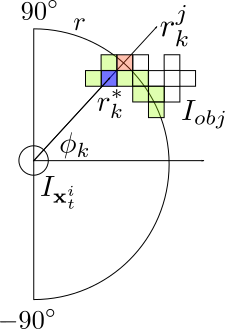
\includegraphics[height=4cm]{../FinalFigures/RayCircleIntersection}\label{subfig:rstar}}
\caption{Visualization of Ray-Circle Intersection}
\label{fig:raycirc}
\end{figure}

We introduce zero mean, additive Gaussian noise with variance $Q$ to $z_t^{i,k}$ to get noisy measurements $\hat{z}_t^{i,k}$:
\begin{equation}
\hat{z}_t^{i,k}=z_t^{i,k}+\mathcal{N}(0,Q).
\end{equation}

\subsubsection{Wall Following}

In this paper we will use wall following to search the environment.  The specifics of this implementation are that it is turned on when $t\in[50,200]$, each robot is equipped with a parity bit to ensure that some robots move in opposite directions, and if the robot happens to get stuck in a loop, wall following will temporarily turn off.

Using wall following to search the environment led to the choice of the odometry motion model, because wall following can be easily implemented with scan data obtained using ray-circle intersection.


\subsubsection{The Odometry Motion Model}

The motion model used was the classic odometry motion model.  
\begin{equation}
\begin{bmatrix}
x_{t}\\
y_{t}\\
\theta_{t}
\end{bmatrix}=\begin{bmatrix}
x_{t-1}\\
y_{t-1}\\
\theta_{t-1}
\end{bmatrix}+\begin{bmatrix}
\hat{\delta}_{t-1}  \cos(\theta_t+\hat{\omega}_t)\\
\hat{\delta}_{t-1}\sin(\theta_t+\hat{\omega}_t)\\
\hat{\omega}_{t-1}
\end{bmatrix},
\label{eq:OdometryMotion}
\end{equation}
where
\begin{eqnarray}
\hat{\delta}_{t-1}&=&\delta_{t-1}-\mathcal{N}(0,\alpha_1\delta_{t-1}^2+\alpha_2\omega_{t-1}^2)\\
\hat{\omega}_{t-1}&=&\omega_{t-1}-\mathcal{N}(0,\alpha_3\delta_{t-1}^2+\alpha_4\omega_{t-1}^2).
\end{eqnarray}

The reverse odometry model is
\begin{equation}
\begin{bmatrix}
x_{t-1}\\
y_{t-1}\\
\theta_{t-1}
\end{bmatrix}=\begin{bmatrix}
x_{t}\\
y_{t}\\
\theta_{t}
\end{bmatrix}-\begin{bmatrix}
\hat{\delta}_t  \cos(\theta_t-\hat{\omega}_{t-1})\\
\delta_{t}\sin(\theta_t-\hat{\omega}_{t-1})\\
\hat{\omega}_{t-1}
\end{bmatrix}
\label{eq:ReverseOdometryMotion}
\end{equation}

\subsubsection{Encounter Detection and Relative Pose}

In place of using a hypothetical camera to determine if robot encounters occur, we use the ray-circle intersection algorithm.  We treat each robot as an object in the binary image, $I$, and if a $(r_k^*,\phi_k)$ is found to coincide with an added robot, and encounter is declared and a relative pose is calculated.  



\subsubsection{The Environment, Robot Trajectories, and Encounters}

Fig. \ref{fig:EnvEnc} contains the test environment and the time when each encounter occurred.  Fig. \ref{subfig:Encvst} shows at what time a robot encountered another, note: only the first encounter is used.

Fig. \ref{subfig:Enc} shows the binary map of the environment, the paths each robot took (colored lines), the point when a robot encounter occurred (dashed gray lines), and where the encounter occurred (thick grey line).
the path each robot took, when a robot encountered another robot, 

\begin{figure}[ht]
\centering
\subfigure[Robot encounters versus time.]{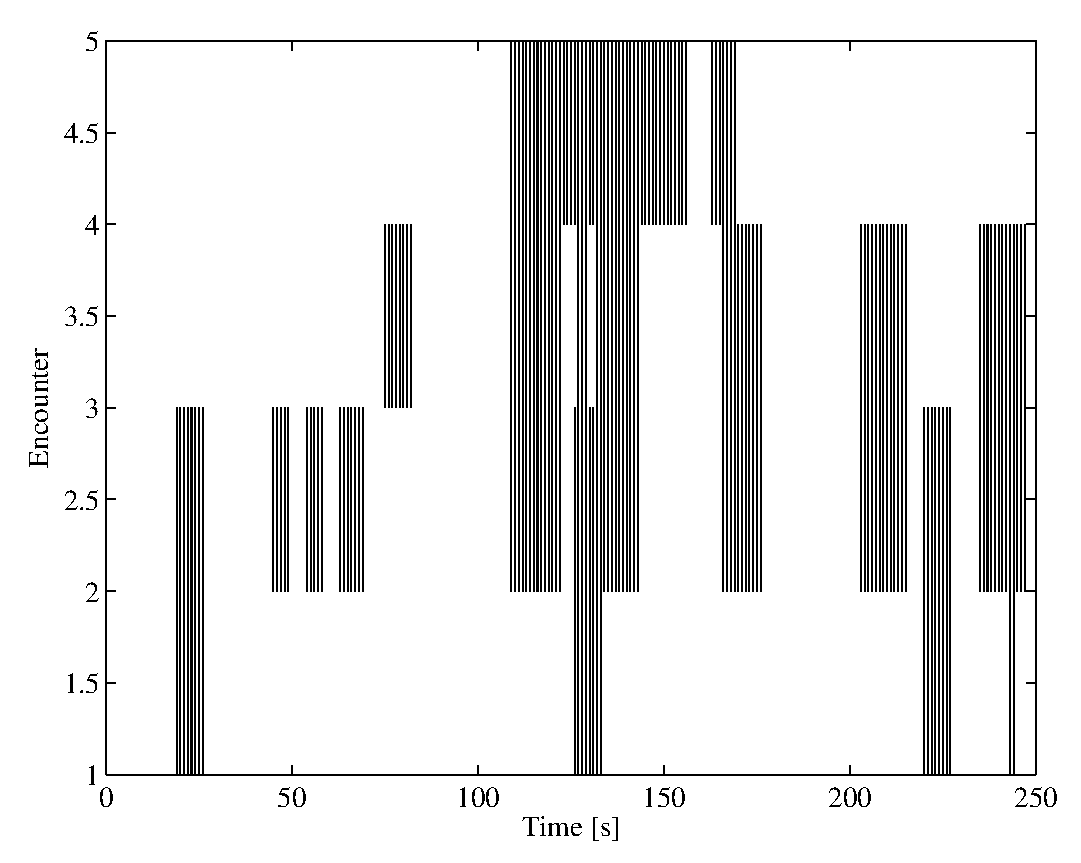
\includegraphics[width=\columnwidth]{../FinalFigures/EncountersTimes}\label{subfig:Encvst}}
\subfigure[The test geometry, robot paths (colored lines), and encounters (dashed gray lines).]{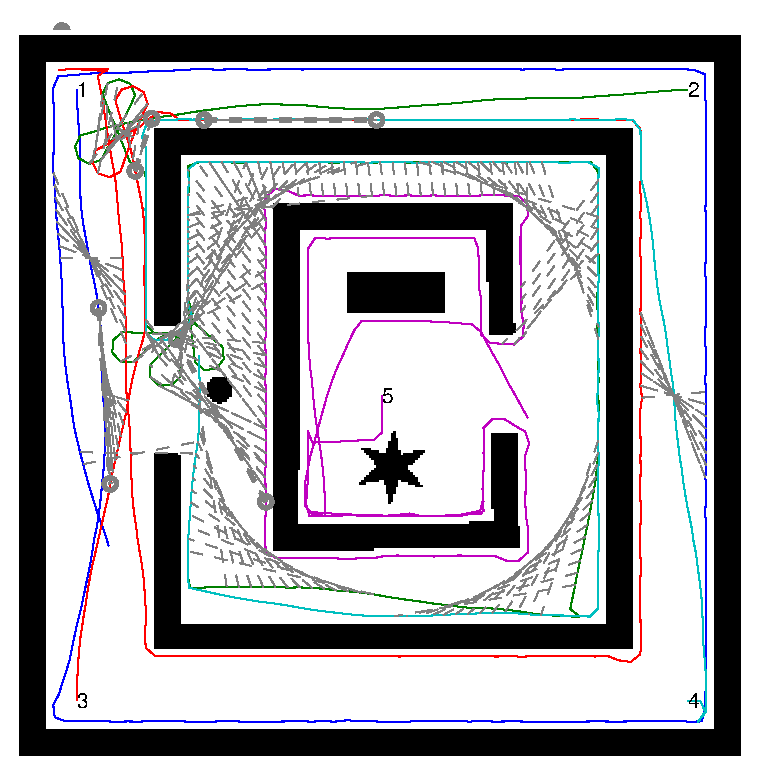
\includegraphics[width=\columnwidth]{../FinalFigures/Encounters}\label{subfig:Enc}}
\caption{Environment geometry, robot paths, and encounters.}
\label{fig:EnvEnc}
\end{figure}








\subsection{The Results}
\label{S:Exp:DataSet}








\begin{frame}
\frametitle{Conclusions}
\begin{itemize}
\item Conclusions:
\begin{itemize}
\item 
\end{itemize}
\item Future work:
\begin{itemize}
\item Decrease 
\item Make it work on Albert B data set
\end{itemize}
\end{itemize}
\end{frame}

\bibliographystyle{plain}
\bibliography{Citations}

%%%%%%%%%%%%%%%%%%%%%%%%%%%%%%%%%%%%%%%%%%%%%%%%%%%%%%%%%%%%%%%%%%%%%%%%%%%%%%%%
\addtolength{\textheight}{-12cm}   % This command serves to balance the column lengths
                                  % on the last page of the document manually. It shortens
                                  % the textheight of the last page by a suitable amount.
                                  % This command does not take effect until the next page
                                  % so it should come on the page before the last. Make
                                  % sure that you do not shorten the textheight too much.

%%%%%%%%%%%%%%%%%%%%%%%%%%%%%%%%%%%%%%%%%%%%%%%%%%%%%%%%%%%%%%%%%%%%%%%%%%%%%%%%



%%%%%%%%%%%%%%%%%%%%%%%%%%%%%%%%%%%%%%%%%%%%%%%%%%%%%%%%%%%%%%%%%%%%%%%%%%%%%%%%



%%%%%%%%%%%%%%%%%%%%%%%%%%%%%%%%%%%%%%%%%%%%%%%%%%%%%%%%%%%%%%%%%%%%%%%%%%%%%%%%





\end{document}
